%!TEX root = paper.tex
%%%%%%%%%%%%%%%%%%%%%%%%%%%%%%%%%%%%%%%%%%%%%%%%%%%%%%%%%%%%%%%%%%%%%%%%%%%%%%%%
\section{Evaluation}
\label{sec:eval}

This section presents the results of the online survey
(§\ref{subsec:survey}) and
investigates the properties of the actual games offered on the
various platforms (§~\ref{subsec:platformproperties}).
The survey covers context-influencing factors including social,
novelty and service-related ones. The platform study scrutinizes
service aspects of context.

\subsection{Online Survey Results}\label{subsec:survey}
The online survey was completed by 488 participants
(91\% self-identified as male, 8\% as female), reporting
ages between 13 and 70 years (quartiles 21, 26, 32; mode 31).
All responses were logged in a timeframe of four days in early 2018.

\subsubsection{Gaming Demographics}
Around 85\% of
participants started playing video games before 10 years of age.
Over 50\% of participants play for 1-3 hours per day.
44\% and 36\% spend 0-20 and 21-50 \$ on games per month, respectively.
Almost 50\% of participants own between 101 and 500 games, and about
15\% report to own 11 to 50 and 501 to 1000 games, respectively.
More than 40\% of participants bought 3 to 10 games in the last
twelve months; slightly more than 45\% claim to have bought
10 to 100 games.



\subsubsection{Social Context Factors And Novelty}

% Where do people learn about new games?
% Is "online" important
% Marketplaces and their influence
% Novelty

When asked to mark all ways of learning about new games, respondents
most prevalently selected ``news on gaming sites'', ``reviews'', and
``friends'' (about 60\% each). Other popular factors include
``live streams'', ``recommendations in online stores'', and
``gaming bundles'' (with 40, 30, and 20\% each). Physical stores
are hardly mentioned.
Digital gaming stores (and among these, \steam) are reported as
the most popular ways of obtaining games. About 85\% of respondents
use digital storefronts. The other proposed selections reach far lower
values: ``third-party key sellers'' hits 35\% , and both ``physical
games from online stores'' and ``physical games from retailers''
are capped around 25\%.


\subsubsection{System Influence Factors}
% Input methods
Almost all participants (97\%) own a PC, the two other most prevalent
gaming systems are smartphones (30\%) and Sony's PlayStation 4 (26\%).
Nintendo's Switch and 3DS as well as Microsoft's XBox One are reported
by 18 to 11\% of participants.
93\% report the PC to be their favorite gaming system, with consoles
favored by 29\%.



\subsubsection{Service Factors}
% important factors for buying new gaming system
% where do you buy
% which online stores
% + specific buying behavior questions:
%   new releases
%   gameplay vs money
%   flat rate
% hindrances

\subsection{Game Platform Properties}\label{subsec:platformproperties}

To complement the subjective gamer results and also provide an
inter-platform comparison, the attention now turns to the service
factors of three gaming platforms: \steam, \gfnow, and \psnow.
Table~\ref{tab:game-stats} provides an overview of the data
collected, showing the number, age, length, and review scores
across platforms.

% %!TEX root = paper.tex

\begin{table}
\caption{Metadata for the \steam, \metacritic, \hltb, \psnow, and \gfnow datasets. Records with a * note include games from other platforms than PC, PlayStation, and GeForce Shield.}
\label{tab:dataset-metadata}
\centering
\begin{tabu}{X[1.5]|X[r]|X[0.7,r]|X}
\toprule
Product & Date generated & \# of records & Method of generation\\
\midrule
\steam & 2015-07-14 & \num{5996} & Steam \& SteamSpy\\
\steam & 2015-10-30 & \num{6769} & Steam \& SteamSpy\\
\steam & 2016-02-06 & \num{7749} & Steam \& SteamSpy\\
\psnow & 2016-02-09 & \num{190} & Official list\\
\gfnow & 2016-02-12 & \num{69} & Manual screen scraping\\
\metacritic & 2016-03-02 & * \num{46197} & Web scraping\\
\hltb & 2016-03-01 & * \num{18433} & Web scraping\\
\bottomrule
\end{tabu}
\end{table}

% %!TEX root = paper.tex

\begin{table*}
\centering
\caption{Overview of datasets. Values with * are 99th percentiles chosen due to unrealistically large outliers.}
\label{tab:dataset-stats}
\begin{tabular}{c|c|r|r|r|r|r|r}
Dataset & Metric & Mean & Min & 1Q & Median & 3Q & Max\\
\hline
\hline
\steam & Number of records & \num{7749} & -- & -- & -- & -- & -- \\
\steam & Owners & \num{218112} & \num{0} & \num{4831} & \num{21740} & \num{107299} & \num{58666968} \\
\steam & players 2weeks & \num{9064} & \num{0} & \num{0} & \num{509} & \num{1526} & \num{7860554} \\
\steam & players forever & \num{138322} & \num{0} & \num{1780} & \num{9408} & \num{51997} & \num{58666968} \\
\steam & Average playtime (forever) & \num{507} & \num{0} & \num{93} & \num{200} & \num{429} & \num{45540} \\
\steam & Median playtime (forever) & \num{246} & \num{0} & \num{36} & \num{101} & \num{216} & \num{67538} \\
\steam & average 2weeks & \num{144} & \num{0} & \num{0} & \num{48} & \num{173} & \num{11387} \\
\steam & median 2weeks & \num{126} & \num{0} & \num{0} & \num{35} & \num{128} & \num{11387} \\
\steam & Price & \num{564} & \num{-1.26} & \num{0.99} & \num{3.39} & \num{7.49} & \num{119.00} \\
\hline
\psnow & Number of records & \num{252} & -- & -- & -- & -- & -- \\
\psnow & Rental fee for 4 hours & \num{3.02} & \num{1.99} & \num{1.99} & \num{2.99} & \num{2.99} & \num{22.99} \\
\psnow & Rental fee for 7 days & \num{5.48} & \num{1.99} & \num{3.99} & \num{4.99} & \num{5.99} & \num{14.99} \\
\psnow & Rental fee for 30 days & \num{8.40} & \num{3.99} & \num{5.99} & \num{6.99} & \num{7.99} & \num{22.99} \\
\psnow & Rental fee for 90 days & \num{12.57} & \num{3.99} & \num{7.99} & \num{8.99} & \num{14.99} & \num{49.99} \\
\hline
\gfnow & Number of records & \num{68} & -- & -- & -- & -- & -- \\
\gfnow & Price & \num{6.98} & \num{0} & \num{0} & \num{0} & \num{13.99} & \num{59.99} \\
\hline
\metacritic & Number of records & \num{45803} & -- & -- & -- & -- & -- \\
\metacritic & User score & \num{6.9} & \num{0} & \num{6.2} & \num{7.3} & \num{8.1} & \num{9.3} \\
\metacritic & Score & \num{69} & \num{8} & \num{62} & \num{72} & \num{79} & \num{96} \\
\hline
\hltb & Number of records & \num{18129} & -- & -- & -- & -- & -- \\
\hltb & Main story length & \num{26} & \num{0.02} & \num{2.5} & \num{6} & \num{12} & * \num{94} \\
\hltb & Main extra length & \num{21} & \num{0.08} & \num{5} & \num{10} & \num{20} & * \num{126} \\
\hltb & Completionist length & \num{28} & \num{0.03} & \num{5} & \num{13} & \num{29} & * \num{250} \\
\hltb & Combined length & \num{13} & \num{0.02} & \num{3} & \num{8} & \num{15} & \num{420} \\
\end{tabular}
\end{table*}

\todo[inline]{PZ: Viele daten, aber welche plattform ist die beste?}


%%%%%%%%%%%%

\begin{table*}
\centering
\caption{Game characteristics on the investigated platforms. Title counts from Web/API scraping, lengths from \hltb, ages and review scores from \metacritic.}
\label{tab:game-stats}
	\begin{tabu}{X[2]|X[r]X[r]X[r]X[r]X[r]X[r]X[r]}
	\toprule
	Service & Titles & Age $\mu$ & Age $\sigma$ & Length $\mu$ & Length $\sigma$ & Score $\mu$ & Score $\sigma$ \\
	\midrule
	\gfnow & $118$ & \SI{3.1}{\year} & \SI{\pm2.3}{\year} & \SI{10.7}{\hour} & \SI{\pm8.2}{\hour} & $73.9$ & $\pm10.1$ \\
	\psnow & $432$ & \SI{4.8}{\year} & \SI{\pm2.4}{\year} & \SI{8.8}{\hour} & \SI{\pm8.8}{\hour} & $71.9$ & $\pm12.0$ \\
	\steam & $14,120$ & \SI{2.5}{\year} & \SI{\pm3.3}{\year} & \SI{7.3}{\hour} & \SI{\pm10.2}{\hour} & $70.6$ & $\pm11.0$ \\
	\bottomrule
	\end{tabu}
\end{table*}


%%%%%%%%%%%%
\subsubsection{Number of Games}

The two cloud
platforms offer a very limited number of games when compared to the
games available on \steam, which itself again only represents a subset
of all games available either on the PC platform (\metacritic lists
$26,420$) or across all platforms ($57,308$). Two
possible, simple explanations for the low game count on the cloud
platforms come to mind: One is that they were launched relatively
recently (2015) in comparison to \steam (2003), leaving little time for
the range of games to grow. Secondly, the choice of games for a cloud
gaming platform is most likely curated by the platform operator for
compatibility and performance reasons. This usability burden shifts to
the end user for digital storefronts like \steam, allowing these
platforms to offer a larger variety of games, including ones that are
very demanding on the hardware. Furthermore, the business models
of the \gls{cg} platforms are still in flux, as described earlier.


%%%%%%%%%%%%
\subsubsection{Game Ages}

The average
game ages appear to be relatively high for all of the investigated
platforms, and particularly so for \psnow. It might be considered a
special case, as it is specifically advertised as a backwards
compatibility for older, pre-PlayStation 4 games that do not run on the
latest Sony platform any more. For \steam, the distribution is
significantly skewed towards recent titles: A quarter of games are less
than a year old, and the median is at $21$ months. The
distribution's tail extends beyond $25$ years due to re-releases
of ``classic'' games on the platform.


%%%%%%%%%%%%
\subsubsection{Game Lengths}
Figure~\ref{fig:gamelengths-violin} shows the distribution of aggregated
game lengths for the three platforms under investigation, and an
``overall'' distribution that includes further platforms and gaming
systems. Among the three platforms, the median reported game
length (approximately \SI{9}{\hour}) is largest for \gfnow. In
contrast to the curated choice of games on the Cloud systems, \steam
also offers shorter and longer games.
The ``overall'' dataset which includes further platforms spans a
yet larger range.


\begin{figure}[!t]
	\centering
	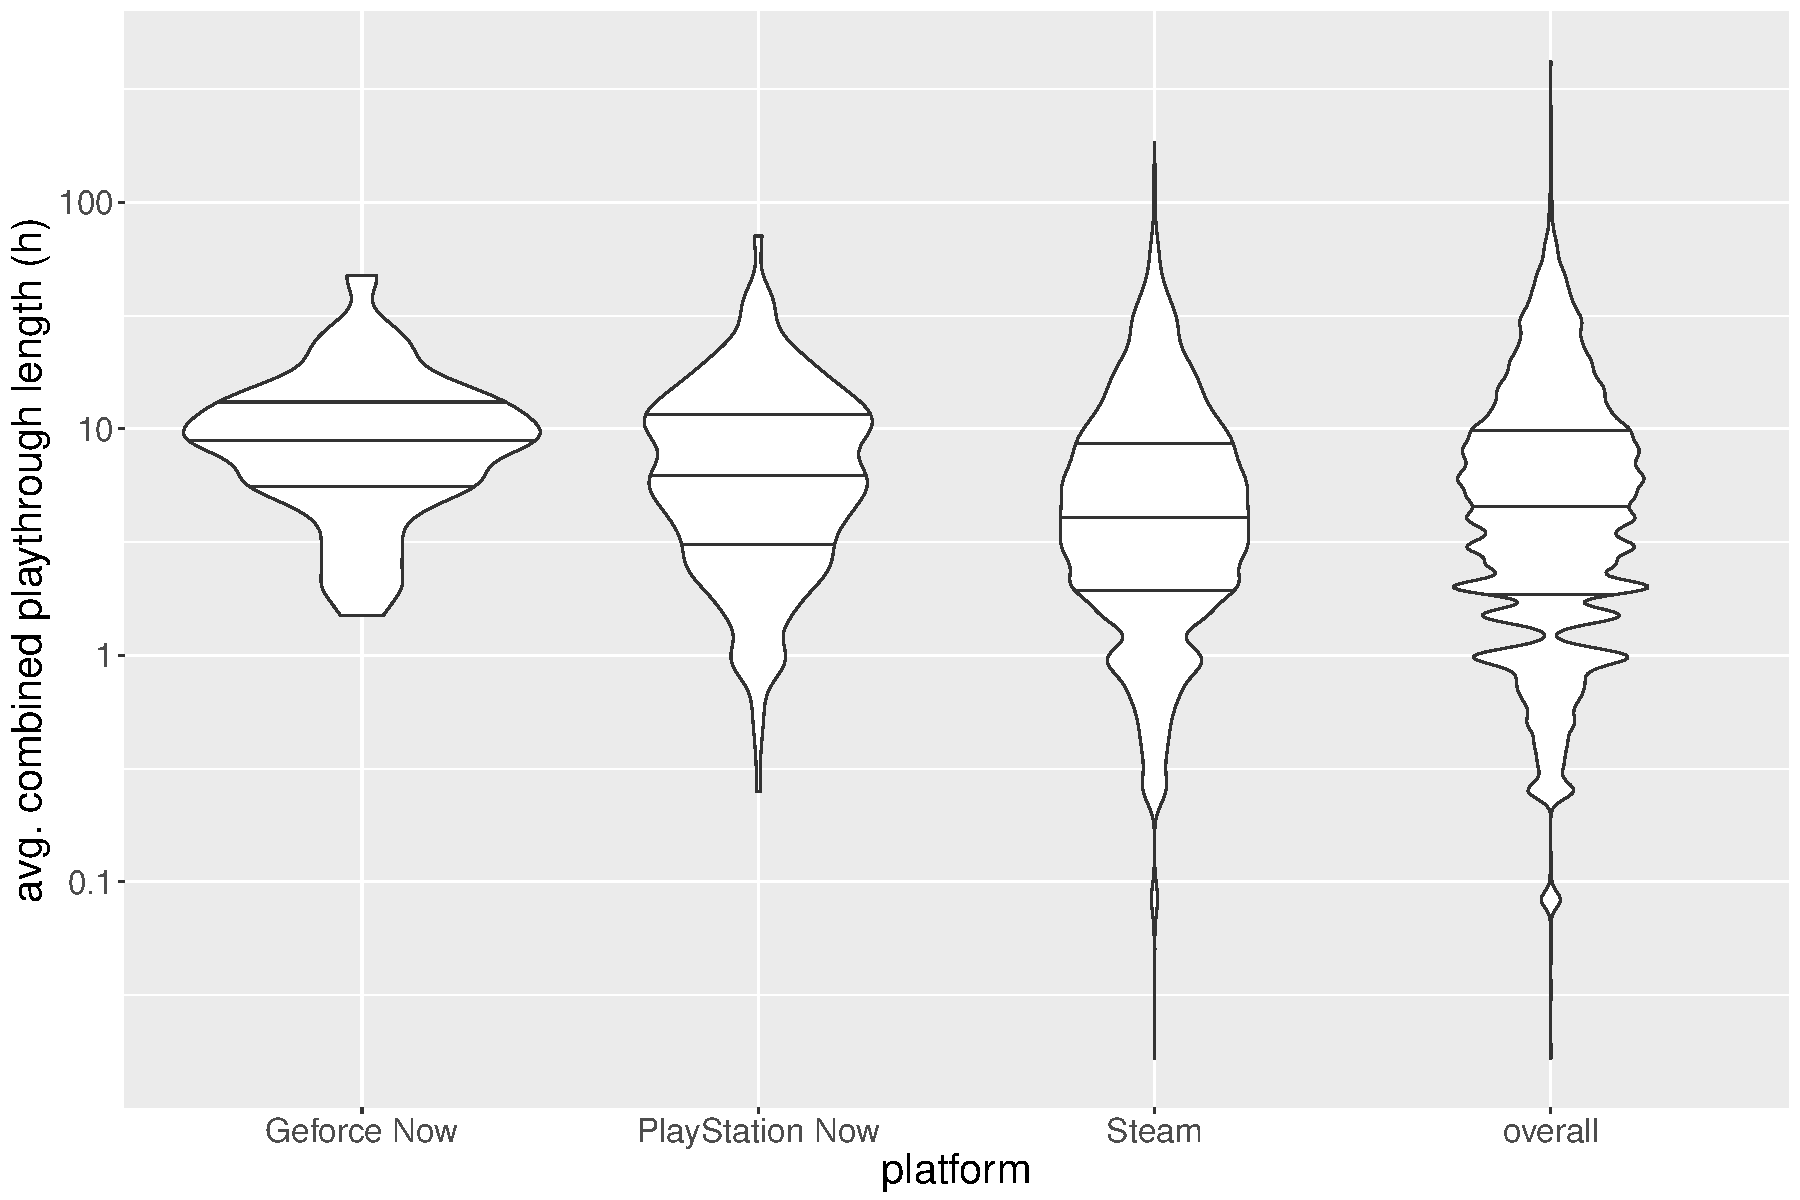
\includegraphics[width=1.0\columnwidth]{images/gamelengths-by-platform-violin.pdf}
	\caption{Violin plot of the per-platform average game lengths from \hltb. Quartiles indicated by horizontal lines.}
%	aggregated over all play styles (raw data source: \hltb).}
\label{fig:gamelengths-violin}
\end{figure}



%%%%%%%%%%%%
\subsubsection{Game Prices}

Trying to compare the prices per game is a difficult endeavor, due to
the mixed approach of the gaming platforms. The \gfnow subscription
gives customers access to a subset of its catalog that can be
extended by purchasing additional games; \gfnowpc and \liquid
on the other hand require the customer to buy games on their
own and pay for the
time spent playing.
\psnow and \psnowpc have a flat rate for all of their catalog.
%Furthermore, the exact subscription and rental modalities as well as prices are adapted over time, and differ between regional markets.
%\todo[inline]{SV:The last sentence was somehow superfluous since variety over time is the case for all of our data. --> erased it.}
At least for \steam, unit prices can be discussed.

\begin{table}
\centering
\caption{Overview of average prices and counts for \steam games.}
\label{tab:steam-price-stats}
\begin{tabu}{X[2]|X[r]X[r]X[r]X[r]X[r]X[r]X[r]X[r]}
	\toprule
	\textbf{Date} & 2015-07 & 2015-10 & 2016-02 & 2016-06 & 2016-09 & 2016-11 & 2017-04 & 2017-10 \\
	\midrule
	\textbf{Average price (€)} & $10.11$ & $8.47$ & $5.65$ & $4.72$ & $8.77$ & $5.33$ & $9.95$ & $8.83$ \\
	\midrule
	\textbf{Standard deviation (€)} & $\pm12.03$ & $\pm9.74$ & $\pm7.88$ & $\pm7.02$ & $\pm10.83$ & $\pm11.08$ & $\pm29.94$ & $\pm12.2$ \\
	\midrule
	\textbf{Number of games} & $5,996$ & $6,769$ & $7,749$ & $9,187$ & $10,191$ & $10,077$ & $11,612$ & $14,120$ \\
	\bottomrule
\end{tabu}
\end{table}


%\begin{figure}[!t]
%	\centering
%	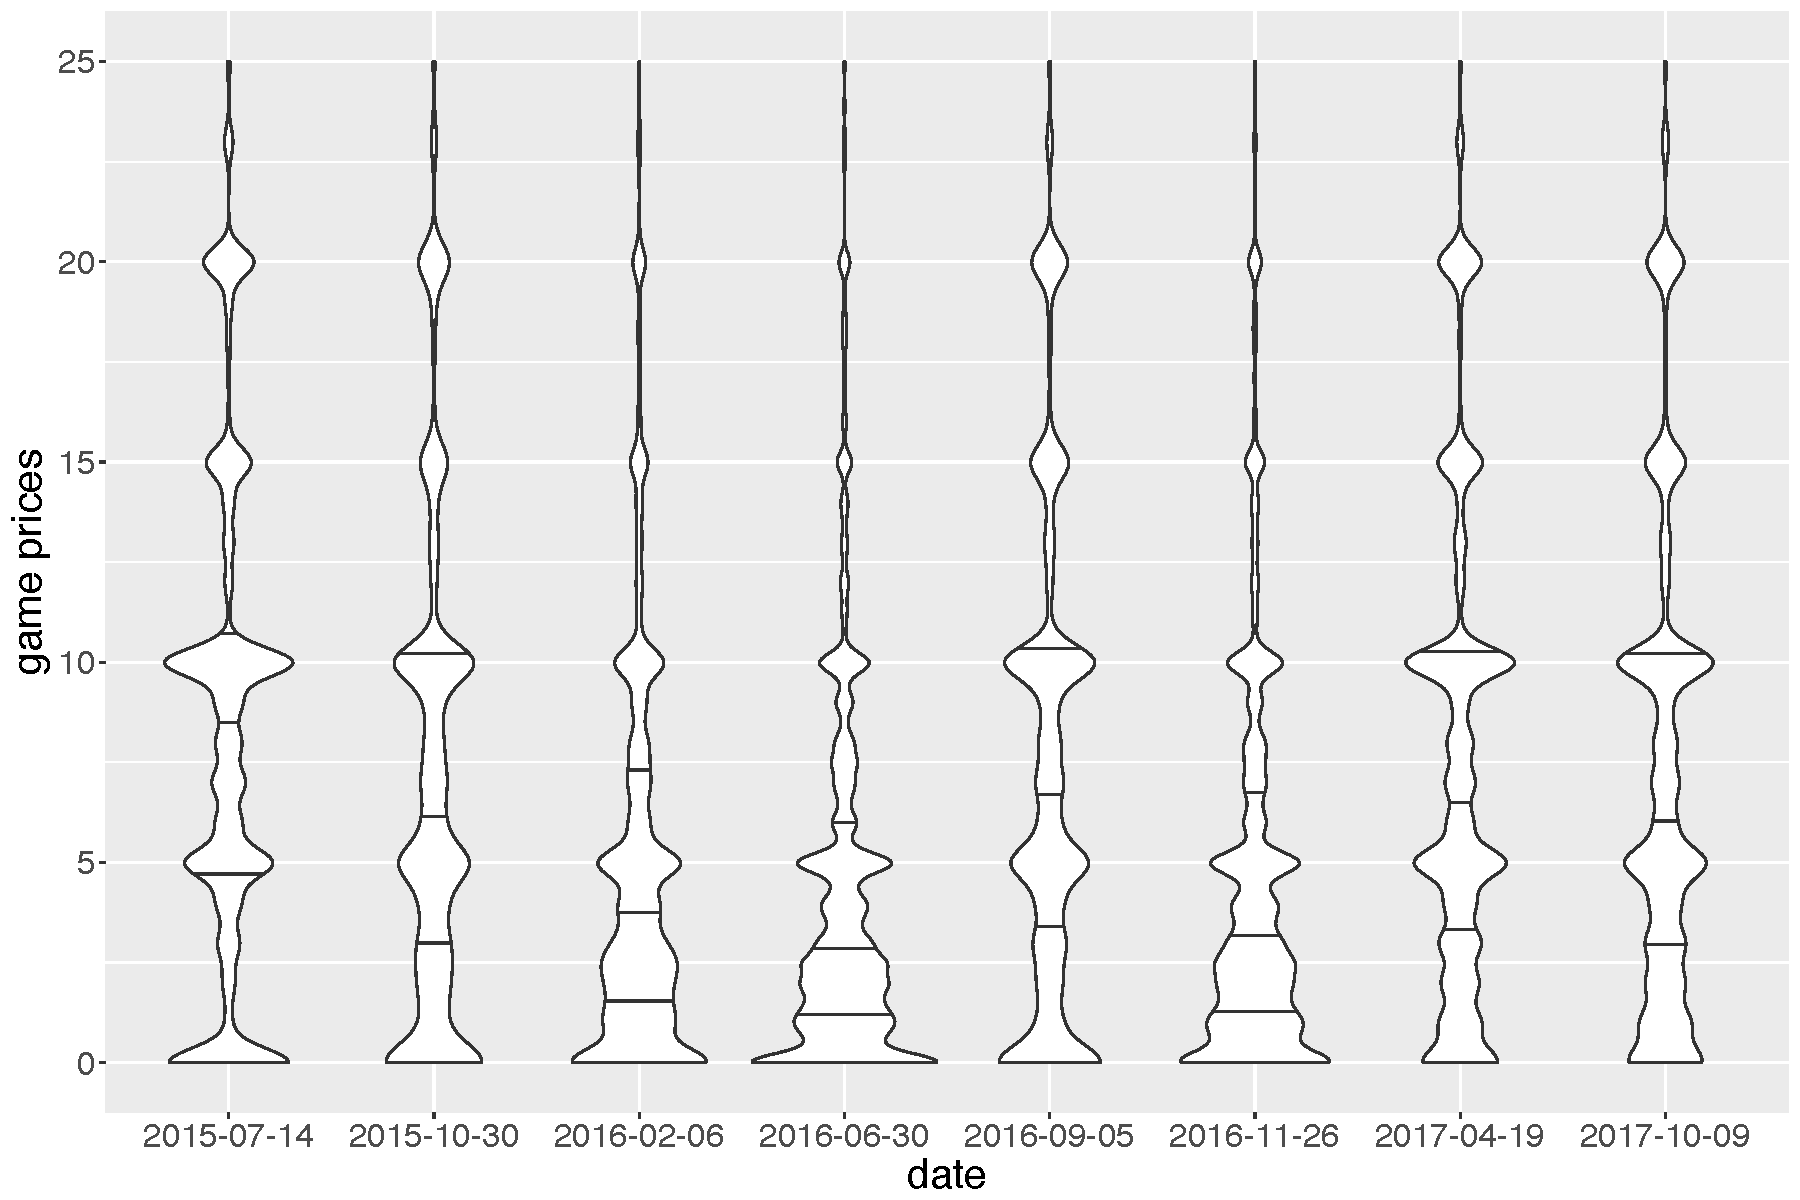
\includegraphics[width=1.0\columnwidth]{images/steam-price-violins-over-time.pdf}
%	\caption{Violin plot of prices of \steam games over time. Quartiles indicated by horizontal lines.}
%\label{fig:steam-price-violins}
%\end{figure}
%# Some modes for 2017-10-09, see steam-prices.R
%#         10% of games are free
%# (18-13)= 5% of games cost  0.99
%# (30-26)= 4% of games cost  2.99
%# (48-36)=12% of games cost  4.99
%# (76-63)=13% of games cost  9.99
%# (87-82)= 5% of games cost 14.99
%# (93-89)= 4% of games cost 19.99
%# The top  6% of games cost more than that


Table~\ref{tab:steam-price-stats} shows the development of average
\steam game prices with standard deviations and the number of available
games for all \steam measurements taken so far, spanning a time interval
of more than two years. As can be seen, the number of games offered
has more than doubled since the first data point, while the average
prices fluctuate over time.
%Figure~\ref{fig:steam-price-violins} complements the table, showing
%smoothed density functions of the game price distributions in \steam's
%store over time in the form of a violin plot.
%Evidently, all distributions have modes (most prominently at nonegative
%multiples of $\text{\texteuro} 5$), and exhibit strong temporal effects.
The variability can be explained by \steam's regular offer of sales
periods with reduced prices. For instance, the shift towards lower
average
prices in February 2016 coincides with a seasonal sales campaign
for Lunar New Year\footnote{\url{http://store.steampowered.com/news/20313/}}.

% Looking at the distributions of game prices, we find that the number of games in the sub \SI{5}]\EUR] category has ... hmm, what ... doubled? ... care to check with R?

%The influence of sales periods can be easily observed in the \acrshort{CDF} of prices in Fig. \ref{fig:steam-prices}, where the data from February was collected during \steam's Lunar New Year Sale.

%\begin{figure}[!t]
%	\centering
%	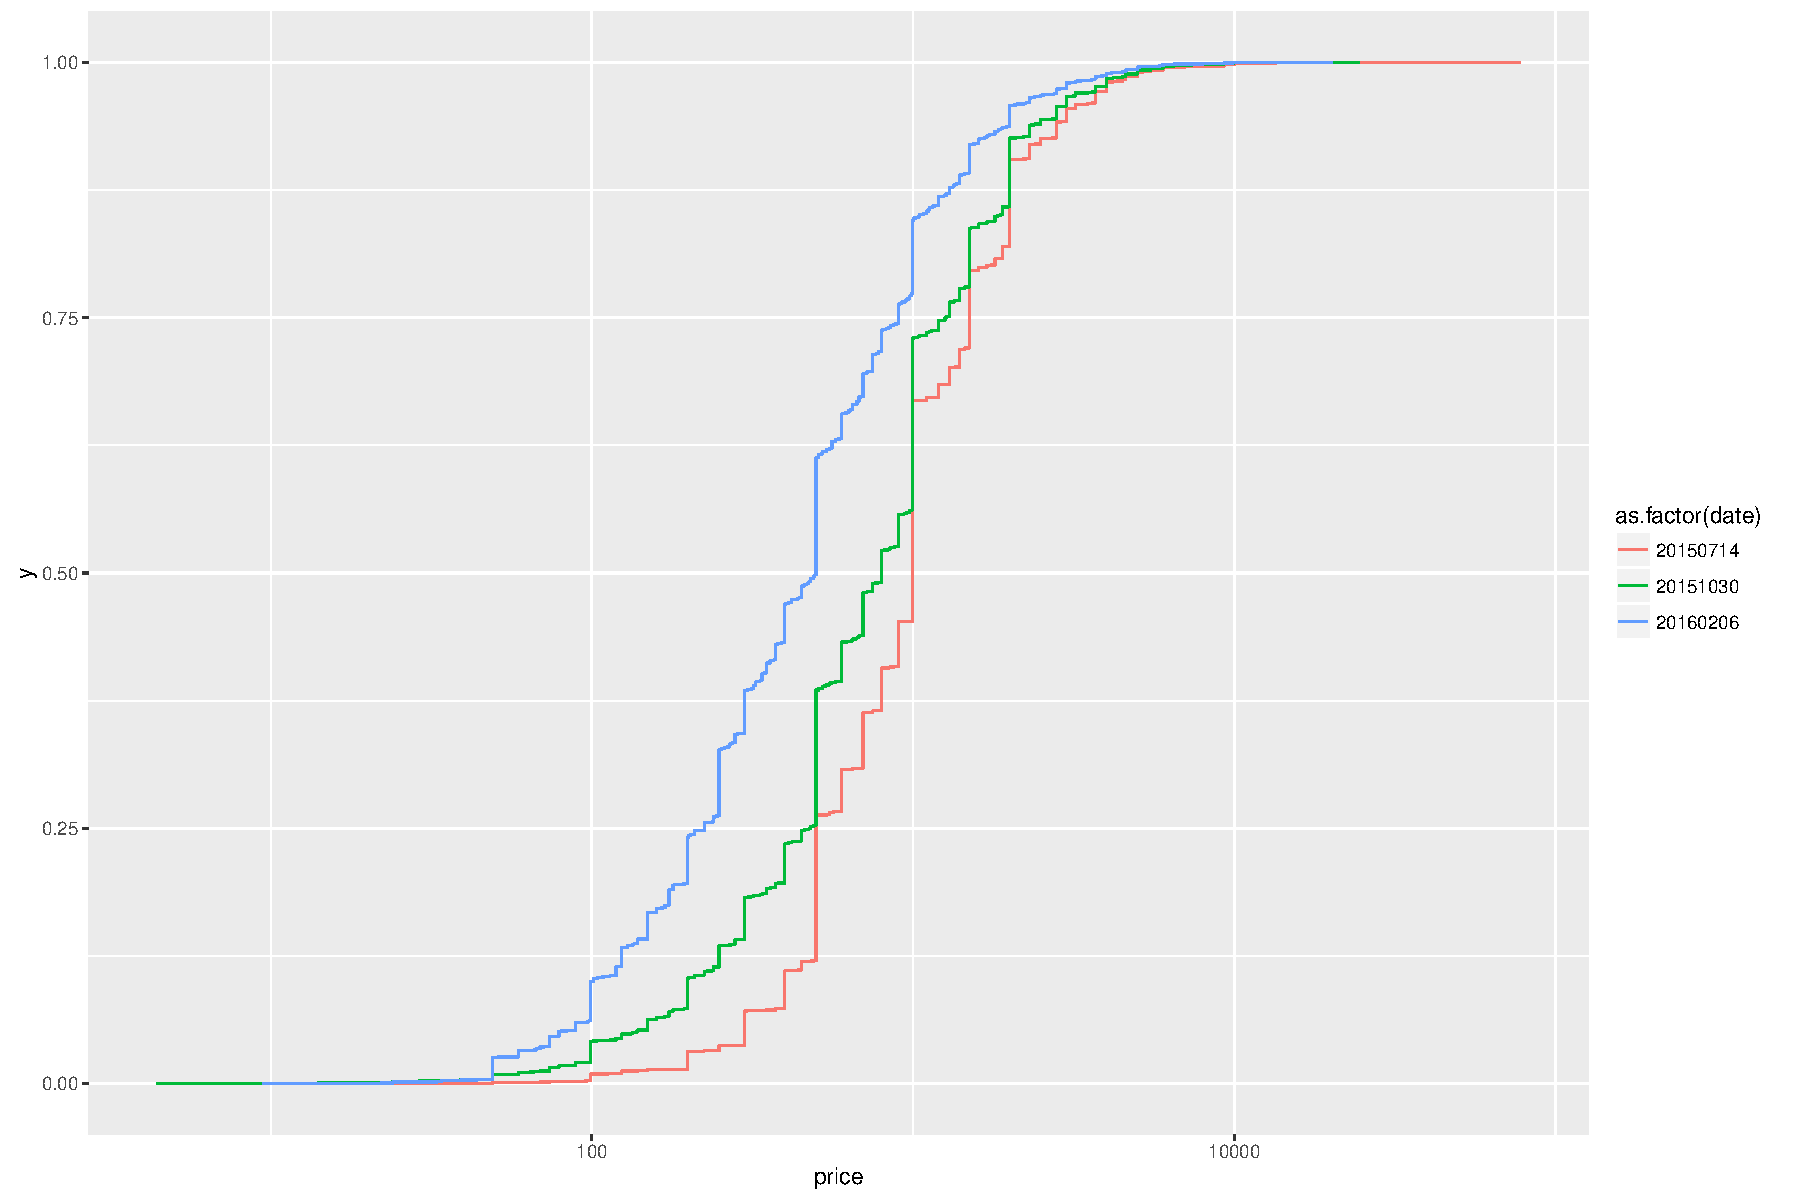
\includegraphics[width=1.0\columnwidth]{images/steam-prices.pdf}
%	\caption{CDF of games on the \steam platform at three distinct dates. The February data was collected in a sales period.}
%\label{fig:steam-prices}
%\end{figure}

\begin{figure}[!t]
	\centering
	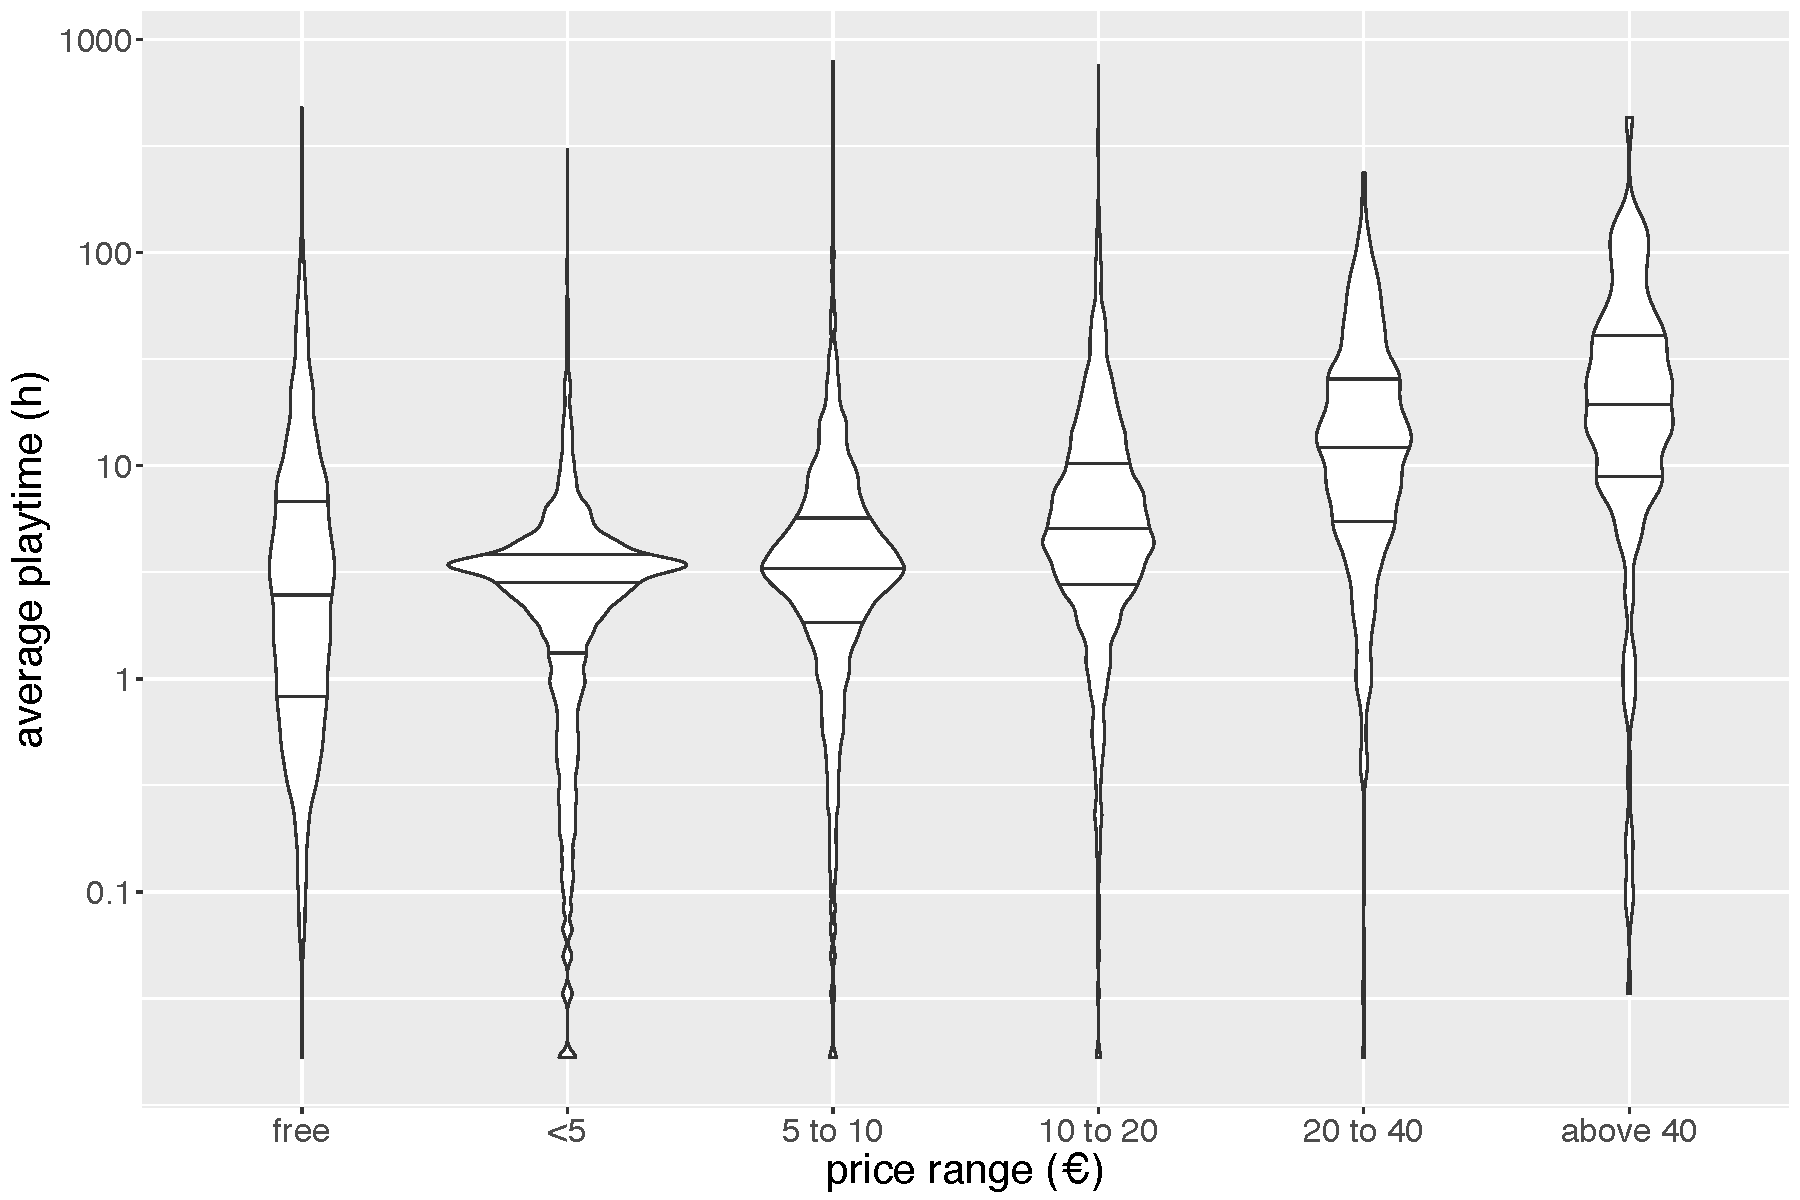
\includegraphics[width=1.0\columnwidth]{images/steam-cost-vs-playtime-non-sale.pdf}
	\caption{Violin plot of the average playtime of \steam games, broadly categorized by their price ranges. The number of games per bin are $1541$, $5269$, $4019$, $2445$, $658$, and $188$. Quartiles indicated by horizontal lines.}
\label{fig:steam-cost-vs-playtime-violin}
\end{figure}

\subsubsection{Price versus Playtime}
Again focusing on \steam,
Figure~\ref{fig:steam-cost-vs-playtime-violin} breaks down the
distribution of average playtimes per game price range. The game price
ranges are chosen so as to roughly separate the prevalent modes of the
price distribution.
Playtime is defined as the time game owners spend playing a game, as
recorded by the \steam platform and scraped from \textit{SteamSpy}.
On the far left in the Figure, playtimes of ``free'' titles
(including free-to-play games with monetization options other than an
upfront payment) span almost the whole playtime range with an
inter-quartile range of 45 minutes to about seven hours.
For games that cost less than $\text{\texteuro} 5$, the mode is around
3.5 hours of playtime, and values are concentrate around it. The
latter is of special interest because it is a recent trend that only
manifested itself in datasets in the last twelve months. It seems that
game producers see this combination of price and playtime as a sweet
spot, as the number of games in this price category grew by a factor of
2.4 in that timeframe --- for comparison, the number of games
increased by 37 percent in the free price range, and roughly doubled
in the other price ranges.

Other than that, the median playtime increases with the price range;
unfortunately, the data does not explain the cause: E.g., more expensive
games might have more playable content, causing the playtime to
increase. Conversely, higher upfront costs may incite players to spend
more time regardless of game quality, thus avoiding regret for the
expense.
% Svenja deleted the following sentence since that can be the case anywhere:
%And still alternatively, there might exist an outside, common reason causing both parameters to increases.
Due to the strong popularity of \steam in \gls{PC} gaming (even physical
retail copies often require using the service nowadays) this set also
gives a good overview of the dimensions of \gls{PC} gaming in general.


%%%%%%%%%%%%
\subsubsection{Review Scores}

The final characteristic presented from the data are game review scores as
given by professional gaming media outlets. This relies on the
\metacritic dataset. This set covers review scores for all current
and historic gaming platforms. The review scores are aggregated to
average scores ranging between $0$ and $100$. Some \metacritic-internal
weighing factors are applied to express the importance of some media
outlets over others.
The average scores seem quite similar across all services, albeit with a
slightly lower $\sigma$ for \gfnow. Figure~\ref{fig:scores-by-platform}
shows the distribution of review scores per platform. Both Cloud
services seem to favor certain score levels, and their averages, medians,
and third quartiles all exceed \steam's.
This could be an effect of the Cloud
systems curating the game offer to focus on highly-rated (and thus
perhaps more attractive) titles. \steam on the other side is a more or
less open platform, where every game publisher can sell their games at
their own volition. The platform operator collects a commission fee for
sales. Consequently, it is reasonable to assume more variation in the
quality of games, which could in turn lead to mixed reviews.
%Cloud gaming platforms have to acquire licenses from the individual games' publishers and therefore have to be selective and curated by nature.
%\todo[inline]{AR: Should we mention other possible effects such as ``Metacritic probably isn't free of bias (gosh!)''?}
% that would only lead to a very, very lengthy off-topic discussion, so probably no

% TODO: include or compare with data from opencritic.com as soon as their API is public/usable

% \begin{figure}[!t]
% 	\centering
% 	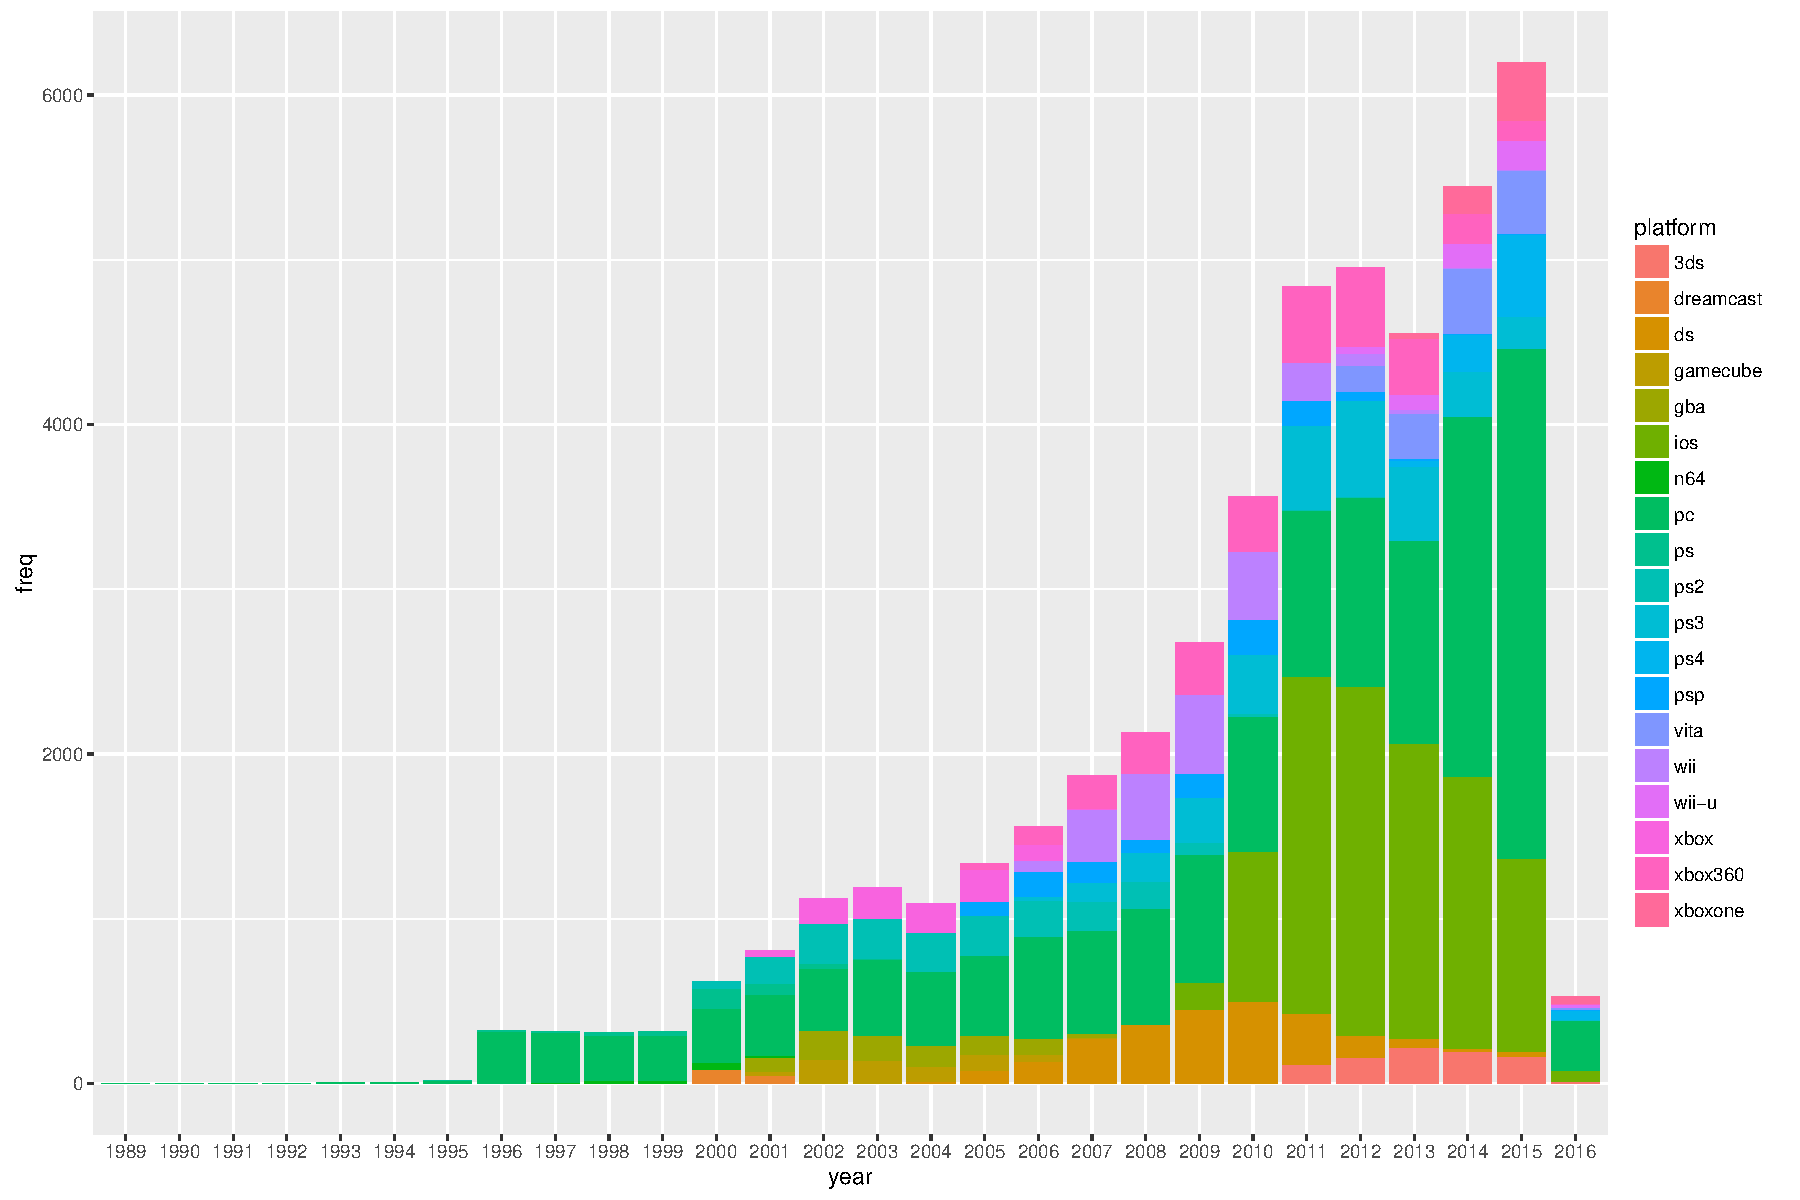
\includegraphics[width=1.0\columnwidth]{images/releases-per-year.pdf}
% 	\caption{Number of game releases per platform according to the Metacritic data.}
% \label{fig:releases-per-year}
% \end{figure}

\begin{figure}[!t]
	\centering
	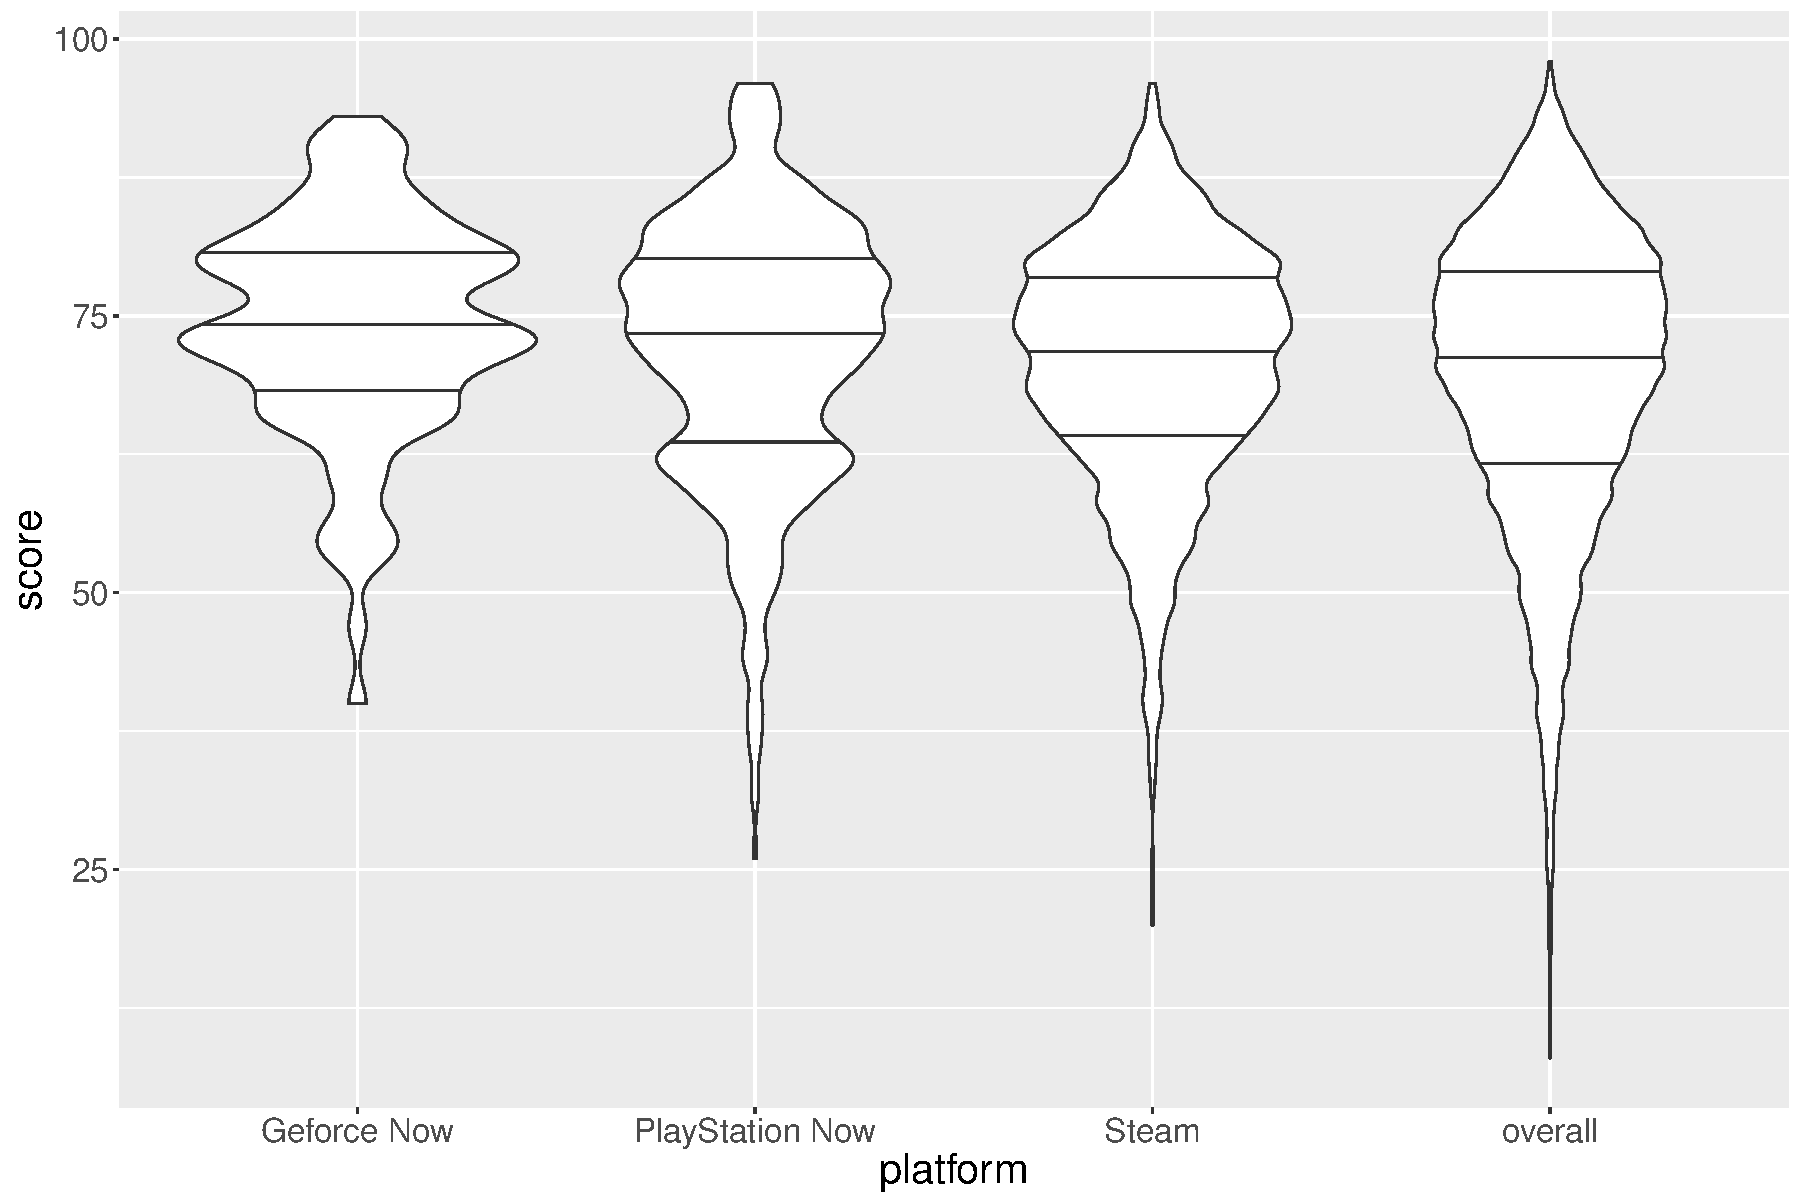
\includegraphics[width=1.0\columnwidth]{images/scores-by-platform-violin.pdf}
	\caption{Violin plot of aggregated review scores per platform. Quartiles indicated by horizontal lines.}
\label{fig:scores-by-platform}
\end{figure}

